% chapters/ch2-sec3a.tex -- 3. Solutions to the Dynamical Equations for Particular Cases of
% Interest; 3.1 Dynamical Behavior at Zero Roll Rate; 3.1.1 Generalized Homogeneous Response;
% 3.1.2 Complete Response to Step Input (PDF 122-149, up to the 3.1.3 heading)
% Corrections applied (corrections/ch2.md): items 1 (Figure 13 caption, silent) and 2 (equation
% (30)) from the 1973 errata sheet (PDF 664); doubt notes D3-D5 and D7 (D6 merged into item 2).
\section{Solutions to the Dynamical Equations for Particular Cases of Interest}\label{ch2:sec:3}

Having given the reader some background from which to proceed, I am going to
compute the properties of some solutions to the dynamical equations which are
of particular interest to the model rocketeer. The presentation will be divided
into two parts: one which will treat rockets having a zero roll rate and a
second which will consider the behavior of models spinning about their
centerlines. Each section will consider the four basic dynamic responses:
homogeneous, step, impulse, and steady-state sinusoidal. It can be shown
mathematically that there is no response that cannot be synthesized by adding
together various combinations of these, so that by investigating the ``basic
four'' a designer can obtain all the information he will ever need about the
dynamic characteristics of his rocket.

I wish to emphasize here that you should \emph{not} become concerned if you
find it difficult to follow the detailed course of each calculation. You will
\emph{not} have to know how to solve the differential equations in order to
design model rockets properly, and the mathematical derivations have been
presented solely for the interest of those readers desiring a rigorous
treatment. What you \emph{should} try to concentrate on are the algebraic
solutions obtained in each case, for it is from these that the response to any
disturbance can be directly computed and it is on them that the dynamical
characteristics of any given model rocket depend.

\subsection{Dynamical Behavior at Zero Roll Rate}\label{ch2:sec:3.1}

\subsubsection{Generalized Homogeneous Response}\label{ch2:sec:3.1.1}

The homogeneous response for generalized initial conditions describes the
motion executed by a rocket in response to some transient disturbance which has
since died away. Since there is no roll coupling only one of the
equations~\eqref{ch2:eq:11} need be solved. The other, which is similar, will
have an analogous solution for its own initial conditions. Suppose that,
throughout this section, we adopt the convention that the rocket is considered
to have been disturbed in yaw alone. In each of the four decoupled problems the
pitching behavior is precisely analogous to the yawing behavior; an analysis of
pitching motion can add nothing to the information already obtained from an
analysis of yawing motion and I have therefore omitted it. All you need
remember on this score is that everything I say about yaw applies also to
pitch.

The equation to be solved for the characteristic yaw response is
\begin{equation*}
I_L \frac{d^{2}\alpha_X}{dt^{2}} + C_2 \frac{d\alpha_X}{dt} + C_1\alpha_X = 0
\end{equation*}
Over a certain range of relative values of $I_L$, $C_1$ and $C_2$ the solution
is known to be of the form
\begin{equation}\label{ch2:eq:15}
\alpha_X = A e^{-Dt}\sin(\omega t + \varphi)
\end{equation}
where $e$ is the base of the \emph{Naperian}, or \emph{natural} logarithm
system and is numerically equal to about 2.718. $t$ denotes time and $A$, $D$,
$\omega$ and $\varphi$ are constants to be determined. By ``time'' I mean the
time elapsed since the observation of the dynamic response has begun, not the
time elapsed since the rocket was launched. To reference
equation~\eqref{ch2:eq:15} to liftoff, call the time elapsed since launch $t'$
and the time interval between launch and the beginning of the observation
$t'_0$. Then replace $t$ in formula~\eqref{ch2:eq:15} by the quantity
$(t' - t'_0)$. $A$ is called the \emph{initial amplitude}, $D$ is defined as
the \emph{inverse time constant}, $\omega$ (not literally an angular velocity
of the rocket's motion) is the \emph{angular frequency} in radians/second (for
time reckoned in seconds), and $\varphi$ is the \emph{phase angle}, or simply
``phase'', in radians. A \emph{radian}, the fundamental natural unit of angle
measure, is approximately equal to 57.3 degrees. The formulae for the time
derivatives of the function described by equation~\eqref{ch2:eq:15}
are:\ednote{The cosine term of the first-derivative formula is printed with the
factor $A\omega D$. The factor $A\omega$ is evidently meant: it is what differentiating
equation~\eqref{ch2:eq:15} gives, and both the second-derivative formula and the
substituted expression that follows are computed with it. Neither the errata
nor the supplements correct this; the formula is kept as printed.}
\begin{align*}
\frac{d\alpha_X}{dt} &= -AD e^{-Dt}\sin(\omega t + \varphi)
  + A\omega D e^{-Dt}\cos(\omega t + \varphi)\\
\frac{d^{2}\alpha_X}{dt^{2}} &= A(D^{2} - \omega^{2}) e^{-Dt}\sin(\omega t + \varphi)
  - 2A\omega D e^{-Dt}\cos(\omega t + \varphi)
\end{align*}
Substituting these relations in the yaw equation gives
\begin{align*}
&I_L A(D^{2} - \omega^{2}) e^{-Dt}\sin(\omega t + \varphi)
  - 2 I_L A\omega D e^{-Dt}\cos(\omega t + \varphi)\\
&\quad - C_2 A D e^{-Dt}\sin(\omega t + \varphi)
  + C_2 A\omega e^{-Dt}\cos(\omega t + \varphi)\\
&\quad + C_1 A e^{-Dt}\sin(\omega t + \varphi) = 0
\end{align*}
Since $Ae^{-Dt}$ is nonzero and appears in every term, we can divide by it and
obtain\ednote{The left edge of this display is cut off on the page: of the
leading $I_L$ of the first line only a fragment of the $I$ and the subscript
$L$ remain, and of the $+$ opening the second line only a sliver. Both are
restored from the preceding display.}
\begin{align*}
&I_L (D^{2} - \omega^{2})\sin(\omega t + \varphi)
  - 2 I_L \omega D\cos(\omega t + \varphi) - C_2 D\sin(\omega t + \varphi)\\
&\quad + C_2\omega\cos(\omega t + \varphi) + C_1\sin(\omega t + \varphi) = 0
\end{align*}
Since sine and cosine vary differently with time the only way in which a
function involving both can be zero for \emph{all} time is for the sine and
cosine terms to sum independently to zero:
\begin{align*}
I_L (D^{2} - \omega^{2})\sin(\omega t + \varphi) - C_2 D\sin(\omega t + \varphi)
  + C_1\sin(\omega t + \varphi) &= 0\\
-2 I_L \omega D\cos(\omega t + \varphi) + C_2\omega\cos(\omega t + \varphi) &= 0
\end{align*}
Dividing the first of these by $\sin(\omega t + \varphi)$, the second by
$\omega\cos(\omega t + \varphi)$, we obtain
\begin{align*}
I_L (D^{2} - \omega^{2}) - C_2 D + C_1 &= 0\\
-2 I_L D + C_2 &= 0
\end{align*}
Solving these two algebraic equations for $D$ and $\omega$ gives
\begin{equation}\label{ch2:eq:16}
D = \frac{C_2}{2 I_L}
\end{equation}
\begin{equation}\label{ch2:eq:17}
\omega = \sqrt{\frac{C_1}{I_L} - \frac{C_2^{2}}{4 I_L^{2}}}
\end{equation}
$A$ and $\varphi$ are now determined from the two \emph{initial conditions}.
Let $\alpha_{X0}$ be the value of $\alpha_X$ at $t = 0$ and let $\Omega_{X0}$
be the value of $d\alpha_X/dt$ at $t = 0$. Setting $t$ to zero in the formulae
for $\alpha_X$ and $d\alpha_X/dt$ results in the following two expressions:
\begin{align*}
\alpha_{X0} &= A\sin\varphi\\
\Omega_{X0} &= -AD\sin\varphi + A\omega\cos\varphi\\
&= -D\alpha_{X0} + A\omega\cos\varphi
\end{align*}
from which
\begin{align*}
\sin\varphi &= \frac{\alpha_{X0}}{A}\\
\cos\varphi &= \frac{D\alpha_{X0} + \Omega_{X0}}{A\omega}
\end{align*}
We now make use of the following trigonometric identity to evaluate $A$ and
$\varphi$:
\begin{equation*}
\frac{\sin\varphi}{\cos\varphi} = \tan\varphi
\end{equation*}
From this we have
\begin{equation}\label{ch2:eq:18}
\tan\varphi = \frac{\alpha_{X0}\,\omega}{D\alpha_{X0} + \Omega_{X0}}
\qquad \text{or} \qquad
\varphi = \arctan\left(\frac{\alpha_{X0}\,\omega}{D\alpha_{X0} + \Omega_{X0}}\right)
\end{equation}
where the notation ``arctan'' has the interpretation, ``that angle whose
tangent is\ldots'' From the expression for $\sin\varphi$ it is also evident
that
\begin{equation}\label{ch2:eq:19}
A = \frac{\alpha_{X0}}{\sin\varphi}
\end{equation}
and thus we have all the information we require to completely describe the
rocket's angular motion. Motion of this kind is called an
\emph{exponentially-damped sinusoid} and its behavior is determined by the
relative values of $I_L$, $C_1$, and $C_2$.

For $C_2 = 0$, the case of \emph{zero damping}, the expression for yaw becomes
\begin{equation*}
\alpha_X = A\sin(\omega_n t + \varphi)
\end{equation*}
where $\omega_n = \sqrt{C_1/I_L}$. $\omega_n$ is known as the \emph{natural
frequency} of the rocket at the given airspeed. The yaw response is
\emph{simple harmonic motion}: sinusoidal oscillations of angular frequency
$\omega_n$ at constant amplitude $A$, as shown in Figure~\ref{ch2:fig:10}. This
motion never really occurs, as there always exists some degree of aerodynamic
damping; it is a so-called \emph{limiting case}, meaning that it is closely
approximated for very small values of $C_2/2I_L$. Such vanishingly small
damping is not desirable, for it means that the oscillations of the rocket will
persist for many cycles without dying away. Under such conditions the rocket
will present a greater average frontal area to the airstream; consequently the
drag will be increased. Since there is also a side force on a yawed or pitched
rocket, some altitude will be lost due to the resulting ``ripple'' in the
flight path as the side force causes a side-to-side movement of the rocket
considered as a whole. For zero damping true alignment would never be regained.

\begin{figure}[htbp]
  \centering
  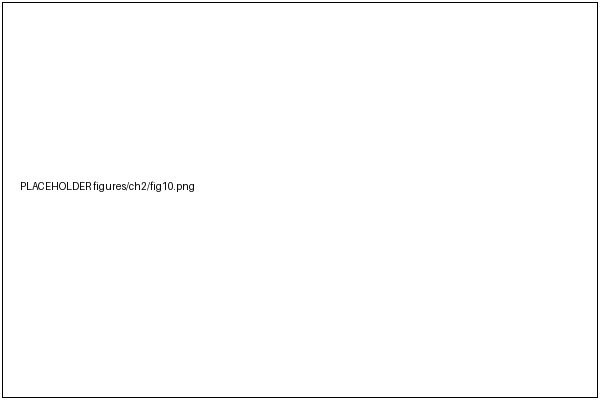
\includegraphics[width=0.8\textwidth,height=0.85\textheight,keepaspectratio]{figures/ch2/fig10.png}
  \caption{Model rocket with zero damping undergoing simple harmonic motion in
  homogeneous response to general initial conditions in yaw. The time to reach
  the first zero, the period of the oscillation, and the relation of the
  initial conditions to the properties of the response are shown. A guide to
  interpreting the graph is presented below it, showing the rocket as it would
  appear at various times if viewed from the negative y axis. This and all
  subsequent calculations of dynamic response presented in this chapter are
  based on the assumption of constant airspeed, so that $C_1$ and $C_2$ do not
  change during the response.}
  \label{ch2:fig:10}
\end{figure}

I might remark at this point that Gurkin's ``Basic Missile Aerodynamic
Stability'' contains references to quantities which are analogous to the
natural frequency and the inverse time constant as defined in the present
treatment. The correspondence between my forms and those of Gurkin is as
follows:
\begin{center}
\begin{tabular}{@{}l c c@{}}
 & \emph{Present Treatment} & \emph{Gurkin Report} \\[6pt]
Natural Frequency & $\omega_n = \sqrt{\dfrac{C_1}{I_L}}$ & $\omega_n = \sqrt{\dfrac{M_\alpha}{I}}$ \\[14pt]
Inverse Time Constant & $D = \dfrac{C_2}{2I_L}$ & $d = \dfrac{M_q}{2I}$ \\
\end{tabular}
\end{center}

For values of $C_1$, $C_2$, and $I_L$ such that
$0 < \frac{C_2^{2}}{4 I_L^{2}} < \frac{C_1}{I_L}$ we have the case of
\emph{underdamped motion}. The oscillations have the appearance of a sine curve
confined within a decaying exponential curve, as shown in
Figure~\ref{ch2:fig:11}. The angular frequency $\omega$ is smaller than the
natural frequency and the amplitude of the oscillations decreases toward zero
with increasing time. The characteristics of almost all model rockets are such
that the homogeneous response will be of this nature at any reasonable
airspeed. This is a desirable type of behavior, for it is in this range of
values of $C_2/2I_L$ that the \emph{quickest restoration} of the rocket to the
intended direction of flight occurs. If we define a \emph{damping ratio}
$\zeta$ by
\begin{equation}\label{ch2:eq:20}
\zeta = \frac{C_2}{2\sqrt{C_1 I_L}}
\end{equation}
and agree to consider straight flight to have been restored when the magnitude
of $\alpha_X$ drops below and never again exceeds 5\% of $A$, we find that the
most rapid restoration occurs when $\zeta = \frac{\sqrt{2}}{2}$, or about
.7071. We therefore have the result
\begin{equation}\label{ch2:eq:21}
\text{optimum damping} \equiv \zeta = \frac{\sqrt{2}}{2}
\end{equation}
Surprisingly, $\zeta > \frac{\sqrt{2}}{2}$ results in a slower restoration.
This is because the decrease in angular frequency becomes more important than
the decrease in the number of cycles required. This decrease in angular
frequency has another, more serious effect: it invalidates one of the
assumptions on which this analysis is based.

\begin{figure}[htbp]
  \centering
  
\includegraphics[width=0.8\textwidth,height=0.85\textheight,keepaspectratio]{figures/ch2/fig11.png}
  \caption{Underdamped characteristic response to general initial conditions in
  yaw. The amplitude of the sinusoidal oscillation is confined within an
  exponentially-decaying ``envelope'' as shown by the dotted line. Also
  illustrated are the relation between the initial conditions and the
  characteristics of the response, the time to reach the first zero, and
  one-half the period required for one full oscillation.}
  \label{ch2:fig:11}
\end{figure}

The reader will recall my references to ``side forces'' and the side-to-side
lateral motion of the rocket which they produce when angular oscillation is
occurring. This lateral motion necessarily involves the presence of velocity
components normal (that is, at right angles) to the intended direction of
flight. Such velocity components, in turn, have the effect of reducing the
apparent yaw angle ``sensed'' by the deflected rocket with the result that the
effective corrective moment is reduced and the frequency of the oscillations is
decreased below that predicted by the linearized theory which considers the CG
of the rocket to undergo no lateral displacement. Luckily, the frequencies at
which most model rockets oscillate are such that the effect of lateral motion
is far too small to be noticeable; \emph{however}, should a given rocket have a
very low frequency of oscillation for its mass (as it would if its damping
ratio were high) the lateral displacements would become very large, so large,
in fact, that the rocket might be very seriously deflected from its intended
vertical trajectory. Too high a damping ratio is thus a dangerous condition and
should be avoided at all costs.

To obtain a clearer picture of the effects of excessive damping, we can examine
the predicted behavior of the rocket as $\zeta$ increases past
$\frac{\sqrt{2}}{2}$. Now we can express $\omega$ in terms of the damping ratio
as
\begin{equation*}
\omega = \omega_n\sqrt{1 - \zeta^{2}}
\end{equation*}
For optimum damping at any airspeed, $\omega$ is just $.7071\,\omega_n$. As
$\zeta$ approaches 1.0, $\omega$ approaches zero, and when a unity damping
ratio is reached, the case of \emph{critical damping}, the motion ceases to be
oscillatory. The form of solution given by equation~\eqref{ch2:eq:15} is no
longer valid.

For the case $\zeta = 1$, corresponding to $C_2^{2}/4I_L^{2} = C_1/I_L$, the
solution to the dynamical equation has the form
\begin{equation}\label{ch2:eq:22}
\alpha_X = (A_1 + A_2 t) e^{-Dt}
\end{equation}
The formulae for the time derivatives of $\alpha_X$ are
\begin{align*}
\frac{d\alpha_X}{dt} &= A_2 e^{-Dt} - D(A_1 + A_2 t) e^{-Dt}\\
\frac{d^{2}\alpha_X}{dt^{2}} &= D^{2}(A_1 + A_2 t) e^{-Dt} - 2A_2 D e^{-Dt}
\end{align*}
Substituting these in the dynamical equation and removing the common factor
$e^{-Dt}$ gives
\begin{equation*}
I_L D^{2}(A_1 + A_2 t) - 2 I_L A_2 D + C_2 A_2 - C_2 D(A_1 + A_2 t)
  + C_1 (A_1 + A_2 t) = 0
\end{equation*}
The terms involving $t$ must sum to zero independently of those not involving
$t$. Imposing this condition, we obtain
\begin{align*}
I_L D^{2} A_1 - 2 I_L A_2 D + C_2 A_2 - C_2 D A_1 + C_1 A_1 &= 0\\
I_L D^{2} A_2 - C_2 D A_2 + C_1 A_2 &= 0
\end{align*}
Removing $A_2$ from the second equation and solving for $D$, we have
\begin{equation*}
D = \frac{C_2}{2 I_L} \pm \sqrt{\frac{C_2^{2}}{4 I_L^{2}} - \frac{C_1}{I_L}}
\end{equation*}
But in this case we already know that $C_2^{2}/4I_L^{2} = C_1/I_L$. The
expression under the radical sign is zero and
\begin{equation*}
D = \frac{C_2}{2 I_L} \qquad \text{as before.}
\end{equation*}
If you substitute $C_2/I_L$ for $D$ in the first equation, you will find that
the terms involving $A_2$ sum to zero.\ednote{The 1973 text reads ``substitute
$C_2/I_L$ for $D$''. The value of $D$ just obtained, $C_2/2I_L$, is evidently
meant: only with it do the terms involving $A_2$ sum to zero and the next
display follow. Neither the errata nor the supplements correct this; the text is
kept as printed.} It is then possible to remove the
now-common factor of $A_1$ and obtain
\begin{equation*}
C_1 - \frac{C_2^{2}}{4 I_L} = 0
\end{equation*}
But if we divide this by $I_L$ we see that it is equivalent to
\begin{equation*}
\frac{C_1}{I_L} - \frac{C_2^{2}}{4 I_L^{2}} = 0
\end{equation*}
which we already know is true, since this is the case for which we are solving.
The differential equation therefore imposes no constraint on $A_1$ and $A_2$;
these are determined by the initial conditions. Setting $t = 0$ in the
expressions for $\alpha_X$ and $d\alpha_X/dt$, we have
\begin{align*}
\alpha_{X0} &= A_1\\
\Omega_{X0} &= A_2 - D A_1
\end{align*}
Then
\begin{equation}\label{ch2:eq:23}
\begin{aligned}
A_1 &= \alpha_{X0}\\
A_2 &= \Omega_{X0} + D\alpha_{X0}
\end{aligned}
\end{equation}
The motion for this case is illustrated in Figure~\ref{ch2:fig:12}. Note that
in this case $\alpha_X$ never crosses to the opposite side of the $t$ axis from
that on which it originates. This behavior is said to exhibit \emph{no
overshoot}. If $\alpha_{X0}$ and $\Omega_{X0}$ are both positive (as shown) or
both negative there will be a single ``peak'' in the curve of yaw angle versus
time before the angular displacement dies away; otherwise it dies away directly
to zero. Despite the fact that $A_2 t$ \emph{increases} as time goes on, the
decay of $e^{-Dt}$ will eventually force the function as a whole to zero.
Critically damped motion is a good deal less desirable than motion of the
oscillatory, underdamped variety. The time to restore alignment is longer and
the rocket will be shifted appreciably to one side by the action of the side
force in one direction only for a substantial period of time. The velocity
involved in this lateral displacement will cause the rocket's flight path to
take a noticeable ``set'', acquiring an inclination away from the intended
vertical trajectory.

\begin{figure}[htbp]
  \centering
  
\includegraphics[width=0.8\textwidth,height=0.85\textheight,keepaspectratio]{figures/ch2/fig12.png}
  \caption{Critically damped characteristic response to general initial
  conditions in yaw. The yaw angle does not oscillate about zero, but
  approaches it asymptotically from above. The relation of the initial
  conditions to the properties of the response has been shown.}
  \label{ch2:fig:12}
\end{figure}

For the class of cases in which $\frac{C_2^{2}}{4 I_L^{2}} > \frac{C_1}{I_L}$,
or $\zeta > 1$, the homogeneous response is of the form
\begin{equation}\label{ch2:eq:24}
\alpha_X = A_1 e^{-\frac{t}{\tau_1}} + A_2 e^{-\frac{t}{\tau_2}}
\end{equation}
where $\tau_1$ and $\tau_2$ are called the \emph{time constants} of the
response. The derivative formulae are
\begin{align*}
\frac{d\alpha_X}{dt} &= -\frac{A_1}{\tau_1} e^{-\frac{t}{\tau_1}}
  - \frac{A_2}{\tau_2} e^{-\frac{t}{\tau_2}}\\
\frac{d^{2}\alpha_X}{dt^{2}} &= \frac{A_1}{\tau_1^{2}} e^{-\frac{t}{\tau_1}}
  + \frac{A_2}{\tau_2^{2}} e^{-\frac{t}{\tau_2}}
\end{align*}
Substituting these expressions in the dynamical equation gives\ednote{The first
term of this display is printed with a bare $A$. The coefficient $A_1$ is evidently meant, as in
the second-derivative formula above and in the other terms in
$e^{-\frac{t}{\tau_1}}$. Neither the errata nor the supplements correct this;
the display is kept as printed.}
\begin{align*}
&I_L \frac{A}{\tau_1^{2}} e^{-\frac{t}{\tau_1}} + I_L \frac{A_2}{\tau_2^{2}} e^{-\frac{t}{\tau_2}}
  - C_2 \frac{A_1}{\tau_1} e^{-\frac{t}{\tau_1}} - C_2 \frac{A_2}{\tau_2} e^{-\frac{t}{\tau_2}}\\
&\qquad + C_1 A_1 e^{-\frac{t}{\tau_1}} + C_1 A_2 e^{-\frac{t}{\tau_2}} = 0
\end{align*}
Those terms involving $A_1 e^{-\frac{t}{\tau_1}}$ and those involving
$A_2 e^{-\frac{t}{\tau_2}}$ must sum to zero independently. The two algebraic equations
thus obtained, with common factors removed, are identical. The form is
\begin{equation*}
\frac{I_L}{\tau^{2}} - \frac{C_2}{\tau} + C_1 = 0
\end{equation*}
Solving for $1/\tau$, we obtain
\begin{equation*}
\frac{1}{\tau} = \frac{C_2}{2 I_L} \pm \sqrt{\frac{C_2^{2}}{4 I_L^{2}} - \frac{C_1}{I_L}}
\end{equation*}
or
\begin{equation*}
\tau = \frac{1}{\dfrac{C_2}{2 I_L} \pm \sqrt{\dfrac{C_2^{2}}{4 I_L^{2}} - \dfrac{C_1}{I_L}}}
\end{equation*}
We choose $\tau_1$, called the \emph{large} time constant, as corresponding to
the negative root. $\tau_2$, the \emph{small} time constant, corresponds to the
positive root:
\begin{equation}\label{ch2:eq:25}
\begin{aligned}
\tau_1 &= \frac{1}{\dfrac{C_2}{2 I_L} - \sqrt{\dfrac{C_2^{2}}{4 I_L^{2}} - \dfrac{C_1}{I_L}}}\\[8pt]
\tau_2 &= \frac{1}{\dfrac{C_2}{2 I_L} + \sqrt{\dfrac{C_2^{2}}{4 I_L^{2}} - \dfrac{C_1}{I_L}}}
\end{aligned}
\end{equation}
The condition $\frac{C_2^{2}}{4 I_L^{2}} > \frac{C_1}{I_L}$ for the validity of
this solution is seen to be the requirement that the square root of a negative
number not occur, and that there be two different time constants. In the same
way, the condition $\frac{C_1}{I_L} > \frac{C_2^{2}}{4 I_L^{2}}$ for the
validity of the sinusoidal solutions was that the square root of a negative
number not occur, and that there be \emph{both} a nonzero $\omega$ and a value
of $D$. The constants $A_1$ and $A_2$ in equation~\eqref{ch2:eq:25}\ednote{The
1973 text reads ``equation (25)''. Equation~\eqref{ch2:eq:24}, in which the
constants $A_1$ and $A_2$ appear, is evidently meant;
equation~\eqref{ch2:eq:25} gives $\tau_1$ and $\tau_2$. Neither the errata nor
the supplements correct this; the reference is kept as printed.} are set by
the initial conditions. Writing $\alpha_{X0}$ and $\Omega_{X0}$ by setting
$t = 0$ in the expressions for $\alpha_X$ and $d\alpha_X/dt$, we obtain
\begin{align*}
\alpha_{X0} &= A_1 + A_2\\
\Omega_{X0} &= -\frac{A_1}{\tau_1} - \frac{A_2}{\tau_2}
\end{align*}
Solving for $A_1$ and $A_2$ gives
\begin{equation}\label{ch2:eq:26}
\begin{aligned}
A_1 &= \frac{\tau_1\alpha_{X0} + \tau_1\tau_2\Omega_{X0}}{\tau_1 - \tau_2}\\[4pt]
A_2 &= \frac{\tau_2\alpha_{X0} + \tau_1\tau_2\Omega_{X0}}{\tau_2 - \tau_1}
\end{aligned}
\end{equation}
A response of this kind is called \emph{overdamped}; its behavior is shown in
Figure~\ref{ch2:fig:13}. Like the critically-damped motion, the overdamped
response has no overshoot; it also decays more slowly than a critically-damped
response. These features make overdamping an extremely hazardous condition.
With overdamping large changes in the flight path almost as severe as those
resulting from neutral static stability can occur if the rocket is disturbed;
in fact, neutral static stability ($C_1 = 0$) is a limiting case of overdamped
motion.

\begin{figure}[htbp]
  \centering
  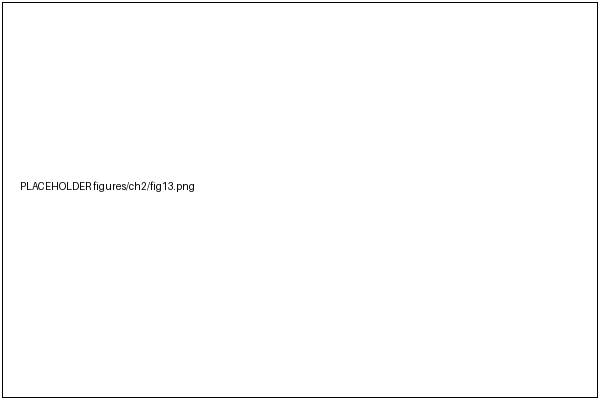
\includegraphics[width=0.8\textwidth,height=0.85\textheight,keepaspectratio]{figures/ch2/fig13.png}
  \caption{Overdamped characteristic response to general initial conditions in
  yaw, showing the relation of the initial conditions to the properties of the
  response. The yaw angle returns to zero more slowly than in the critically
  damped case, and in the limit of infinite damping ratio the rocket would
  instantly lose its initial yaw rate and remain ``stuck'' at the initial yaw
  angle $\alpha_{X0}$ as if encased in very thick glue or tar.}
  \label{ch2:fig:13}
\end{figure}

A statically unstable rocket (one whose corrective moment coefficient is
\emph{negative}) also responds to a disturbance in a manner described by
equation~\eqref{ch2:eq:24}. Although the damping ratio is undefined for
negative $C_1$, both time constants and both initial amplitudes are computable
from equations~\eqref{ch2:eq:25} and~\eqref{ch2:eq:26}. If you carry out these
computations you will find that $\tau_1$ becomes negative when $C_1$ is less
than zero, so that $e^{-\frac{t}{\tau_1}}$ becomes $e$ raised to a \emph{positive
power}. The ``exponential mode'' associated with $\tau_1$ thus
\emph{increases} with time, meaning that the yaw angle of the rocket grows
larger and larger as time goes on. This is the dynamic description of a
statically unstable rocket ``going ape''. Such an unstable, or
\emph{divergent}, response is illustrated in Figure~\ref{ch2:fig:14}. The
statement ``$C_1$ must be greater than zero'' for a rocket to be stable is the
dynamic equivalent of the statement ``the center of pressure must lie aft of
the center of gravity''. No matter what the phraseology employed to say it,
positive static stability is the prime requirement of a successful rocket
design.

\begin{figure}[htbp]
  \centering
  
\includegraphics[width=0.8\textwidth,height=0.85\textheight,keepaspectratio]{figures/ch2/fig14.png}
  \caption{Characteristic response of a statically unstable rocket to general
  initial conditions in yaw, showing the relation of the initial conditions to
  the properties of the response. The yaw angle does not return to zero, but
  rather \emph{increases} with time, so that the rocket will eventually flip
  end over end and execute completely unpredictable maneuvers. Negative static
  stability is thus a dangerous condition and should always be avoided when
  designing model rockets.}
  \label{ch2:fig:14}
\end{figure}

\subsubsection{Complete Response to Step Input}\label{ch2:sec:3.1.2}

Suppose that a rocket which has been flying straight and true in calm air
suddenly breaks into a region of the sky in which a wind of constant velocity
is blowing parallel to the ground (such a phenomenon is called a
\emph{discontinuous wind shear}). Or suppose such a rocket having four fins,
each with a control tab, experiences a condition whereby the tabs on two
opposing fins suddenly deflect an equal amount in the same direction. Finally,
consider what would happen if such a rocket experiences an engine or engine
mounting malfunction in which the thrust line suddenly assumes an angle
relative to the rocket's centerline. Occurrences such as these fall into the
category of \emph{step inputs}, a name derived from the graphical appearance of
their variation with respect to time. The moment-versus-time graph of a
representative step function appears in Figure~\ref{ch2:fig:15}.

\begin{figure}[htbp]
  \centering
  
\includegraphics[width=0.8\textwidth,height=0.85\textheight,keepaspectratio]{figures/ch2/fig15.png}
  \caption{A step disturbance of intensity $M_s$. Before $t = 0$ the yawing
  moment is zero; after $t = 0$ it is $M_s$ dyn-cm.}
  \label{ch2:fig:15}
\end{figure}

A step input, for the purposes of this analysis, takes the form of an applied
moment whose value is zero before a given time and whose value is a constant
after that time. The time at which the ``step'' occurs is considered to be
$t = 0$. With this convention we can define a step input in yaw mathematically
as follows:
\begin{align*}
f_x(t) &= 0 \qquad (t < 0)\\
f_x(t) &= M_s \qquad (t \ge 0)
\end{align*}
A function of this form is, of course, an idealization. You couldn't expect to
observe a perfectly sharp step in any real physical quantity; nevertheless an
analysis of the response of a rocket to a step input (hereafter abbreviated
``step response'') provides the designer with information of considerable
value, for step-response analysis is one of the two standard methods of
defining the relative ease with which a given rocket can be displaced from true
alignment with its intended flight path.

We recall that the differential equation describing the response of a
non-rolling rocket to forcing in yaw is
\begin{equation*}
I_L \frac{d^{2}\alpha_X}{dt^{2}} + C_2 \frac{d\alpha_X}{dt} + C_1\alpha_X = f_x(t)
\end{equation*}
Substituting our definition of the step input, we have
\begin{subequations}\label{ch2:eq:27}
\begin{align}
I_L \frac{d^{2}\alpha_X}{dt^{2}} + C_2 \frac{d\alpha_X}{dt} + C_1\alpha_X
  &= 0 \qquad (t < 0)\label{ch2:eq:27a}\\
I_L \frac{d^{2}\alpha_X}{dt^{2}} + C_2 \frac{d\alpha_X}{dt} + C_1\alpha_X
  &= M_s \qquad (t \ge 0)\label{ch2:eq:27b}
\end{align}
\end{subequations}
Now I stipulated that the rocket under consideration be flying straight and
evenly at the time the step is applied. This is equivalent to stating that the
yaw angle and all its time derivatives are zero for all time preceding the
application of the step. The rocket is said to be in a \emph{rotationally
quiescent state} for $t < 0$ and you can see that such a condition identically
satisfies equation~\eqref{ch2:eq:27a}.

Equation~\eqref{ch2:eq:27b} is solved by the \emph{sum} of the characteristic
and particular responses (cf. Section~\ref{ch2:sec:2.4}). The characteristic
response, obtained in Section~\ref{ch2:sec:3.1.1}, is given by
equation~\eqref{ch2:eq:15}, equation~\eqref{ch2:eq:22}, or
equation~\eqref{ch2:eq:24}, depending on the value of the quantity
$\frac{C_1}{I_L} - \frac{C_2^{2}}{4 I_L^{2}}$. The particular response in this
case is
\begin{equation}\label{ch2:eq:28}
\alpha_X = K
\end{equation}
where $K$ is a constant. Since a constant cannot (by its very definition) vary
with time, all of its time derivatives are zero. Upon substitution of $K$ for
$\alpha_X$, equation~\eqref{ch2:eq:27b} thus becomes
\begin{equation*}
C_1 K = M_s
\end{equation*}
from which
\begin{equation}\label{ch2:eq:29}
K = M_s/C_1
\end{equation}
The complete step-response for the cases in which
$\frac{C_1}{I_L} > \frac{C_2^{2}}{4 I_L^{2}}$ is therefore\ednote{Equation~\eqref{ch2:eq:30}
corrected per the 1973 errata sheet; the 1973 equation read
$\alpha_X = A e^{-Dt}\sin(\omega t + \varphi)$, without the particular-response
term $M_s/C_1$ of equation~\eqref{ch2:eq:29}, which the initial-condition
expressions that follow and equations~\eqref{ch2:eq:33} and~\eqref{ch2:eq:35}
include.}
\begin{equation}\label{ch2:eq:30}
\alpha_X = A e^{-Dt}\sin(\omega t + \varphi) + \frac{M_s}{C_1}
\end{equation}
where $D$ is given by equation~\eqref{ch2:eq:16} and $\omega$ by
equation~\eqref{ch2:eq:17}. As in Section~\ref{ch2:sec:3.1.1}, the values of
$A$ and $\varphi$ are determined by the initial conditions. It can be shown
that, for a rocket quiescent before the application of the step input, both the
angular displacement $\alpha_X$ and the angular velocity $d\alpha_X/dt$ are
zero at $t = 0$. Now setting time equal to zero in the expressions for
$\alpha_X$ and $d\alpha_X/dt$ results in
\begin{equation*}
\alpha_{X0} = A\sin\varphi + \frac{M_s}{C_1}
\end{equation*}
and
\begin{equation*}
\Omega_{X0} = A(\omega\cos\varphi - D\sin\varphi)
\end{equation*}
which, when $\alpha_{X0}$ and $\Omega_{X0}$ are set equal to zero, give us
\begin{equation*}
A\sin\varphi = -\frac{M_s}{C_1}
\end{equation*}
and
\begin{equation*}
D\sin\varphi = \omega\cos\varphi
\end{equation*}
From the second of these we can obtain
\begin{subequations}\label{ch2:eq:31}
\begin{equation}\label{ch2:eq:31a}
\varphi = \arctan\left(\frac{\omega}{D}\right)
\end{equation}
from which we have
\begin{equation}\label{ch2:eq:31b}
A = -\frac{M_s}{C_1\sin\varphi}
\end{equation}
\end{subequations}

The motion described by equation~\eqref{ch2:eq:30} is an exponentially-damped
sinusoid which oscillates about the offset horizontal line
$\alpha_X = M_s/C_1$. For the case of zero damping it is simple harmonic motion
about $\alpha_X = M_s/C_1$ as shown in Figure~\ref{ch2:fig:16}. The undamped
oscillation varies in magnitude from zero to $2M_s/C_1$, starting from zero
with a zero angular velocity at time $t = 0$. The underdamped case, which is
again the desirable one for rocket behavior, is given in
Figure~\ref{ch2:fig:17}. The angular displacement, again starting with zero
magnitude and slope, ``homes in'' in an oscillatory manner on the displaced
axis at $M_s/C_1$. It is of interest to compute the value of the first
``peak'' of such an oscillation and the time at which it occurs, since this
information is useful in evaluating the merits of a given rocket design with
respect to dynamic behavior.

\begin{figure}[htbp]
  \centering
  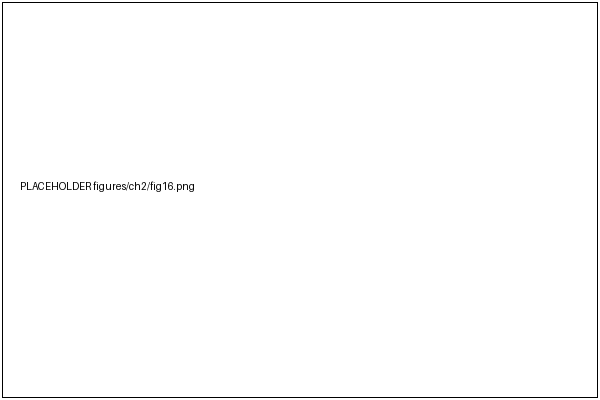
\includegraphics[width=0.8\textwidth,height=0.85\textheight,keepaspectratio]{figures/ch2/fig16.png}
  \caption{Undamped response to a step disturbance in yaw. The rocket
  oscillates indefinitely about the yaw angle $M_s/C_1$. Also shown are the
  maximum yaw angle and the time at which it is first attained.}
  \label{ch2:fig:16}
\end{figure}

\begin{figure}[htbp]
  \centering
  
\includegraphics[width=0.8\textwidth,height=0.85\textheight,keepaspectratio]{figures/ch2/fig17.png}
  \caption{Underdamped response to a step disturbance in yaw. After a
  sufficiently long time the model will come to rest at the yaw angle
  $M_s/C_1$. Also shown are the maximum yaw angle and the time at which it
  occurs.}
  \label{ch2:fig:17}
\end{figure}

The first peak will occur at the smallest \emph{nonzero} value of time for
which the angular velocity is zero, i.e., for which $d\alpha_X/dt = 0$.
Performing the operation of differentiation and setting the resulting
expression equal to zero gives us
\begin{equation*}
-AD e^{-Dt}\sin(\omega t + \varphi) + A\omega e^{-Dt}\cos(\omega t + \varphi) = 0
\end{equation*}
from which, dividing by $Ae^{-Dt}$, we obtain
\begin{equation*}
-D\sin(\omega t + \varphi) + \omega\cos(\omega t + \varphi) = 0
\end{equation*}
This requires that
\begin{equation*}
\tan(\omega t + \varphi) = \frac{\omega}{D}
\end{equation*}
Now if you take the inverse trigonometric function of both sides of this
equation, you will wind up with
\begin{equation*}
\omega t + \varphi = \arctan\left(\frac{\omega}{D}\right)
\end{equation*}
or
\begin{equation*}
t = \frac{\arctan\left(\frac{\omega}{D}\right) - \varphi}{\omega}
\end{equation*}
But since $\varphi = \arctan(\omega/D)$, the only solution obtainable from this
equation is $t = 0$. While this is indeed a solution (our initial condition,
$\Omega_X = 0$, is based on it), it does not identify the time of occurrence of
the first peak. The \emph{general} solution for the time at which the $n$th
peak occurs is obtained by introducing the trigonometric identity
\begin{equation*}
\tan(\omega t + \varphi + n\pi) = \tan(\omega t + \varphi) \qquad (n \text{ an integer})
\end{equation*}
\emph{Now} if we take the inverse trigonometric functions we obtain
\begin{equation*}
\omega t + \varphi + n\pi = \arctan\left(\frac{\omega}{D}\right)
\end{equation*}
from which
\begin{equation*}
t = \frac{n\pi}{\omega}
\end{equation*}
The first peak occurs at the time associated with the value $n = 1$:
\begin{subequations}\label{ch2:eq:32}
\begin{equation}\label{ch2:eq:32a}
t = \frac{\pi}{\omega}
\end{equation}
The value of $\alpha_X$ at the first peak is computed by substituting this
value of $t$ into equation~\eqref{ch2:eq:30}:
\begin{equation*}
\bigl.\alpha_X\bigr|_{t = \frac{\pi}{\omega}} = A e^{-\frac{\pi D}{\omega}}\sin(\pi + \varphi) + \frac{M_s}{C_1}
\end{equation*}
By the use of the trigonometric identity
\begin{equation*}
\sin(\pi + \varphi) = -\sin\varphi
\end{equation*}
and equation~\eqref{ch2:eq:31b} this may be simplified to read
\begin{equation}\label{ch2:eq:32b}
\bigl.\alpha_X\bigr|_{t = \frac{\pi}{\omega}} = \frac{M_s}{C_1}\left[1 + e^{-\frac{\pi D}{\omega}}\right]
\end{equation}
\end{subequations}
A look at Figure~\ref{ch2:fig:17} will reveal that this value of $\alpha_X$
represents the greatest magnitude the angular displacement attains during the
step-response. Since the magnitude of the displacement \emph{decreases} as
$C_1$ increases, we conclude that a large value of $C_1$ will reduce the
severity of a rocket's step response.

In the case where the values of $C_1$, $C_2$, and $I_L$ are such that a
condition of critical damping exists the complete step-response is given by
\begin{equation}\label{ch2:eq:33}
\alpha_X = (A_1 + A_2 t) e^{-Dt} + \frac{M_s}{C_1}
\end{equation}
where $D$ is again given by equation~\eqref{ch2:eq:16}. Applying the initial
conditions, we have
\begin{align*}
\alpha_{X0} &= A_1 + \frac{M_s}{C_1}\\
&= 0
\end{align*}
and
\begin{align*}
\Omega_{X0} &= A_2 - D A_1\\
&= 0
\end{align*}
from which we obtain
\begin{subequations}\label{ch2:eq:34}
\begin{align}
A_1 &= -\frac{M_s}{C_1}\label{ch2:eq:34a}\\
A_2 &= -D\,\frac{M_s}{C_1}\label{ch2:eq:34b}
\end{align}
\end{subequations}
A critically-damped step-response is shown in Figure~\ref{ch2:fig:18}.

\begin{figure}[htbp]
  \centering
  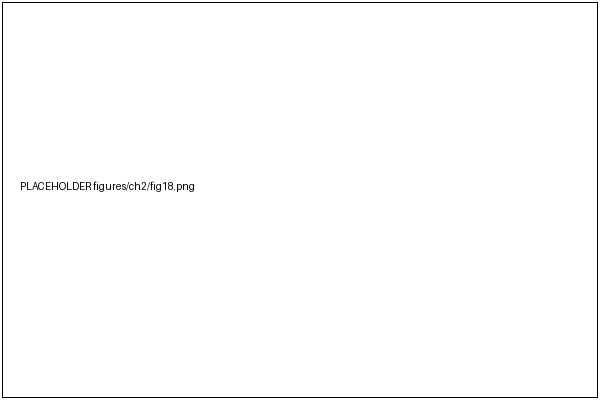
\includegraphics[width=0.8\textwidth,height=0.85\textheight,keepaspectratio]{figures/ch2/fig18.png}
  \caption{Critically damped response to a step disturbance in yaw. The yaw
  angle approaches a value of $M_s/C_1$ asymptotically from below.}
  \label{ch2:fig:18}
\end{figure}

The complete expression for an \emph{overdamped} step response is
\begin{equation}\label{ch2:eq:35}
\alpha_X = A_1 e^{-\frac{t}{\tau_1}} + A_2 e^{-\frac{t}{\tau_2}} + \frac{M_s}{C_1}
\end{equation}
where $\tau_1$ and $\tau_2$ are given by equations~\eqref{ch2:eq:25}. In this
case the imposition of initial conditions results in the expressions
\begin{align*}
\alpha_{X0} &= A_1 + A_2 + \frac{M_s}{C_1}\\
&= 0
\end{align*}
and
\begin{align*}
\Omega_{X0} &= -\frac{A_1}{\tau_1} - \frac{A_2}{\tau_2}\\
&= 0
\end{align*}
from which we have
\begin{subequations}\label{ch2:eq:36}
\begin{equation}\label{ch2:eq:36a}
A_1 = -\frac{M_s\tau_1}{C_1(\tau_1 - \tau_2)}
\end{equation}
and
\begin{equation}\label{ch2:eq:36b}
A_2 = \frac{M_s\tau_2}{C_1(\tau_1 - \tau_2)}
\end{equation}
\end{subequations}
Figure~\ref{ch2:fig:19} illustrates an overdamped step-response.

\begin{figure}[htbp]
  \centering
  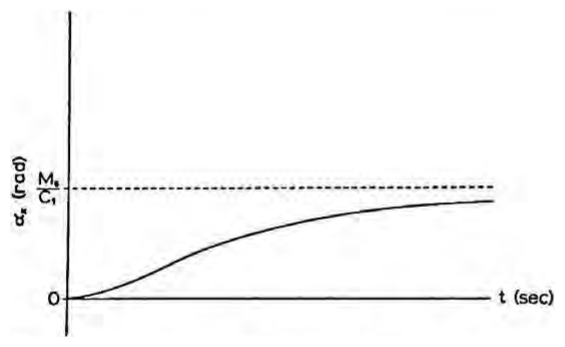
\includegraphics[width=0.8\textwidth,height=0.85\textheight,keepaspectratio]{figures/ch2/fig19.png}
  \caption{Overdamped response to a step disturbance in yaw. The yaw angle
  $M_s/C_1$ is again approached asymptotically from below, but more slowly than
  is the case for the critically damped response.}
  \label{ch2:fig:19}
\end{figure}

The critically-damped and overdamped step responses are both slower than the
underdamped response, and in this sense the former are somewhat less sensitive
to step inputs than the latter. Consider what would happen, though, if the step
were to arise, persist for a considerable length of time, and then drop to zero
again. An overdamped rocket would \emph{also} be slow in \emph{returning} to
true alignment from a yaw angle of nearly $M_s/C_1$ radians. Moreover, since
overdamped responses exhibit no overshoot, the deflection of the flight path
from the vertical would be substantially greater than in the case of
underdamped motion. It is therefore best to decrease a rocket's sensitivity to
step inputs by the use of a large corrective moment coefficient rather than
high damping.
